\hspace{1em} Transport is the key enabler of economic growth and social development 
of countries around the World. European Union (EU) is one of the most developed regions in the World, 
and it is a good example on how the development of logistics improves quality of life. 
\begin{figure}[h]
    \centering
    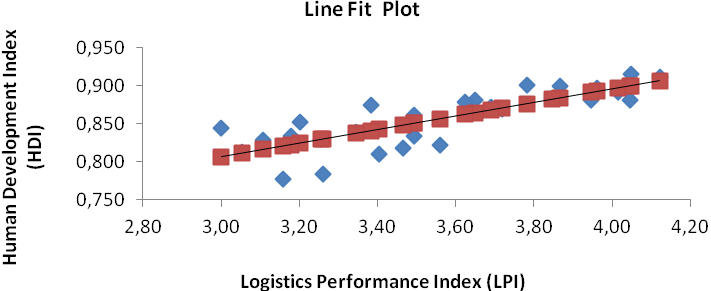
\includegraphics[width=0.8\textwidth]{figures/correlation_HDI_LPI.png}
    \caption{The correlation between the Logistics Performance Index (LPI) and the Human Development\cite{HDIvsLPI}}
    \label{fig:correlation_HDI_LPI}
\end{figure}


As shown in in figure \ref*{fig:correlation_HDI_LPI} the relationship between European Union country 
logistics performance and quality of life is strong. However, transportation is also 
a net emmiter of \ce{CO2} in EU. According to the European Environment Agency (EEA) report domestic
transport is responsible for 29.17\% of total \ce{CO2} emissions in 2022\cite{EEA}. And yet the trend of 
domestic transport utilisation is still increasing.This is a clear indicator that transportation is sub-optimal and requires
 improvements in order to reduce the impact on environment. 

Public transport is seen a solution on how to tackle the problem of increasing \ce{CO2} emissions.
Efficient and reliable public transport systems can reduce the number of cars used, thus reducing 
the load on public roads and mitigating unnecessary accident risks. However, to acheive that
it there are some dificult challenges that need to be addressed. SOme of the most important aspects
that keep people in their car are:
    unreliable schedules,
    long waiting times,
    inconvenient routes,
    high ticket prices,
    overloaded buses

In the scope of this research some of the most important hurdles for public transport will be addressed.
The main focus of this paper will be put on increasing the efficiency of bus dispatching and scheduling.
By optimising the route and schedule, the number of buses utilised in the fleet can be reduced and 
the size of bus sent on route can be adjusted to the number of passengers expected. 
By doing so, the costs of operations should decrease thus, making public transportation services more
affordable and attractive to the society.

To optimise the dispatching and scheduling neural network models will be used. The models will
be trained on historical data on sales of tickets in bus stops. The developed model will be
used to predict the number of passengers in bus stops in the future. The decision on the size of the bus
to dispatch and stations to include in the route will be made by the dispatcher, but with real time
advice from the neural network model. 
